\documentclass{beamer}

\newcommand{\week}{Financial Markets 5 of 8}

\title{Bonds 4: Risk and Term Structure of Interest Rates}
\subtitle{Mishkin Chapter 6}
\author{Econ 357}
\date{\week}

% Reference the shared preamble
\input{preamble}

% Set the footer -- change 
\setbeamertemplate{footline}{
  \leavevmode%
  \vspace{2ex}
  \hbox{%
    % Left box: Econ 457
    \begin{beamercolorbox}[wd=.4\paperwidth,ht=2.5ex,dp=1ex,left]{author in head/foot}%
      \hspace{1em}Econ 357
    \end{beamercolorbox}%
    % Middle box: Week
    \begin{beamercolorbox}[wd=.2\paperwidth,ht=2.5ex,dp=1ex,center]{date in head/foot}%
      \centering\week
    \end{beamercolorbox}%
    % Right box: Slide numbers
    \begin{beamercolorbox}[wd=.4\paperwidth,ht=2.5ex,dp=1ex,center]{date in head/foot}%
      \hfill\insertframenumber{} 
    \end{beamercolorbox}%
  }%
  \vskip0pt%
}

\begin{document}

\frame{\titlepage}

\begin{frame}
    \frametitle{Outline for Financial Markets}
        \begin{enumerate}
            \item Financial Market Returns
            \item Bonds 1: Discounting, Prices and Yields
            \item Bonds 2: Nominal v. Real Interest Rates, Supply and Demand
            \item Bonds 3: Market for Money
            \item \fbox{Bonds 4: Risk and Term Structure}
            \item Equities 1: Dividend Discount Model
            \item Equities 2: P/E Ratio
            \item Equities 3: Theories of Stock Pricing
            
        \end{enumerate}
\end{frame}


\begin{frame}
    \frametitle{Outline for Today's Lecture}
    \begin{enumerate}
        \item Default Risk
        \item Taxes and Municipal Bonds
        \item The Treasury Yield Curve
        \begin{itemize}
            \item Explanations for slope of yield curve
            \item Is the yield curve a recession indicator?
        \end{itemize}
    \end{enumerate}

\end{frame}

\begin{frame}[t]
    \frametitle{Review}

    \textbf{Prices and Yields}
    \begin{itemize}
        \item Bond prices and yields are inversely related
        \item When the bond yield is equal to the coupon, the bond price is equal to \$100.   Bonds are typically priced at \$100 when they are issued, then the prices rise (fall) as yields fall (rise).  The yield is an indication of the expected return on the bond.
        \item A premium bond (price $>\$100$) has a yield below the coupon rate, and is one that you prefer to have bought when it was issued (because you would have benefitted from the price appreciated).   A discount bond (price $<\$100$) has a yield above the coupon rate, is one that you prefer to buy now (because the price is lower, and the prospective returns are therefore higher.)
    \end{itemize}


\end{frame}

\begin{frame}[t]
    \frametitle{Review}

    \textbf{Supply and Demand for Bonds}
    \begin{itemize}
        \item Demand (Households / Investors): wealth, expected return, risk, liquidity
        \item Supply (Corporations / US Treasury): profit opportunities, government deficits
    \end{itemize}
    
    \textbf{Supply and Demand for Money}
    \begin{itemize}
        \item Demand (Checking account v. Investment Account): downward sloping with bond interest rate on y-axis
        \item Supply (Federal Reserve): vertical line
    \end{itemize}

\end{frame}

\begin{frame}
    \frametitle{1. Default Risk}
    \section{Default Risk}

    \textbf{Definitions}
    \begin{itemize}
        \item Risk-free rate: The interest rate on US Treasury bonds, which are assumed to have no default risk.
        \item Default premium: The difference between the interest rate on a corporate bond and the risk-free rate.
    \end{itemize}
    \vspace{1em}
    
        \textbf{Discussion}
    \begin{itemize}
        \item While US Treasuries are used as the risk-free rate, remember that there is a lot of price risk in Treasuries, which is to say the prices can go up and down.
        \item The default premium is not equal to the interest rate on a corporate bond.
    \end{itemize}

\end{frame}

\begin{frame}
    \frametitle{1. Default Risk}

    \centering
    
\includegraphics[width=\textwidth]{Econ357/figures/02_mkts_3_history2.png}

\end{frame}

\begin{frame}
    \frametitle{1. Default Risk}

    \centering
    
\includegraphics[width=\textwidth]{Econ357/figures/02_mkts_3_history3.png}

\end{frame}

\begin{frame}[t]
    \frametitle{1. Default Risk}
    \framesubtitle{Credit Rating Agencies}

    \begin{itemize}
        \item Credit rating agencies assess the \textbf{creditworthiness} of
        corporations, governments, and other borrowers.

        \item The three major U.S. rating agencies are:
        \begin{itemize}
            \item \textbf{Moody's}
            \item \textbf{S\&P Global Ratings}
            \item \textbf{Fitch Ratings}
        \end{itemize}

        \item Ratings summarize the agency's assessment of the likelihood
        that a borrower will meet its debt obligations.

        \item Ratings range from \textbf{investment grade} to
        \textbf{speculative grade} (``junk'').

        \item Lower-rated bonds generally must offer \textbf{higher yields}
        to compensate investors for greater perceived credit risk.
    \end{itemize}

\end{frame}

\begin{frame}[t]
    \frametitle{1. Default Risk}
    \framesubtitle{Credit Ratings}

    \vspace{-2em}
    \begin{center}
    \end{center}
    \begin{tblr}{
      colspec = { Q[l,wd=3cm, font=\footnotesize] |Q[c,wd=3cm, font=\footnotesize] | Q[c,wd=4cm, font=\footnotesize] }
    }
    Moody's & S\&P and Fitch & Examples \\
    \midrule
    \SetCell[c=3]{c}\textbf{ Investment Grade} \\
    Aaa, Aa1, Aa2, Aa3 & AAA, AA+, AA & Microsoft, J\&J \\
    A1, A2, A3 & A+, A, A- & JPM, UBS \\
    Baa1, Baa2, Baa3 & BBB+, BBB & Boeing, Occidental Petroleum \\
    \SetCell[c=3]{c} \textbf{High Yield (also: Below Investment Grade or Junk)} \\
    Ba1, Ba2, Ba3 & BB+, BB, BB- & Carnival Corporation \\
    B1, B2, B3 & B+, B, B- & Caesars Entertainment \\
    \bottomrule
    \end{tblr}

\end{frame}




\begin{frame}[t]
    \frametitle{1. Default Risk}
    \framesubtitle{Default Premium}

    A bond's \textbf{default premium} is defined as the difference between the bond yield and the yield on a similar maturity US Treasury bond.

    $$\text{Default Premium} = \text{Bond Yield} - \text{US Treasury Yield}$$

    \begin{itemize}
        \item Be careful to only compare bonds with similar maturities
        \item The default premium is not equal to the default risk. 
    \end{itemize}

\end{frame}

\begin{frame}[t]
    \frametitle{1. Default Risk }
    \framesubtitle{Fallen Angels and Rising Stars}

    \begin{itemize}
        \item Bond yields tend to increase when a company's ratings are downgraded.   A company that is downgraded from investment grade to high yield is known as a "fallen angel".  
        \item Conversely, bond yields tend to fall when a company's ratings are upgraded.  A company that is upgraded from high yield to investment grade is known as a "rising star."
    \end{itemize}
    \vspace{1em}

    \textbf{Example}: Occidental Petroleum was initially an investment grade company (rated A in 2017), it was then downgraded to high yield (BB) in 2020, and was subsequently upgraded back to investment grade (BBB-) in 2023.

\end{frame}

\begin{frame}[t]
    \frametitle{1. Default Risk}
    \framesubtitle{Occidental Petroleum, 4.625\% of 2045}

    \centering
    
\includegraphics[width=0.8\textwidth]{Econ357/figures/02_mkts_5_oxy.png}
    % https://www.tradingview.com/chart/?symbol=SWB%3AOPCC

\end{frame}

\begin{frame}[t]
    \frametitle{1. Default Risk }

     % https://fixedincome.fidelity.com/ftgw/fi/FIYieldTable?popupMode=Y&yldTabSelected=H

    Yields and Default Premiums
    (Indictative, not exact)

    \vspace{-2em}
    \begin{center}
    \end{center}
    \begin{tblr}{
      colspec = { Q[l,wd=5cm] Q[c,wd=2cm] Q[c,wd=2cm] }
    }
    \toprule
    Index & Yields & Default Premium \\
    \midrule
    US Treasury, 5y & 4.9\% &  na\\
    AA Rated Corp Bonds & 5.4\% & ? \\ 
    Baa / BBB Rated Corp Bonds & 7.2\% & ? \\
    BB Rated & 8\% & ? \\
    CCC Rated & 13\% & ? \\
    \bottomrule
    \end{tblr}
    
\end{frame}    

\begin{frame}[t]
    \frametitle{1. Default Risk }
    \framesubtitle{Credit Ratings}

    \begin{columns}
        \begin{column}{0.3\textwidth}
            \centering
            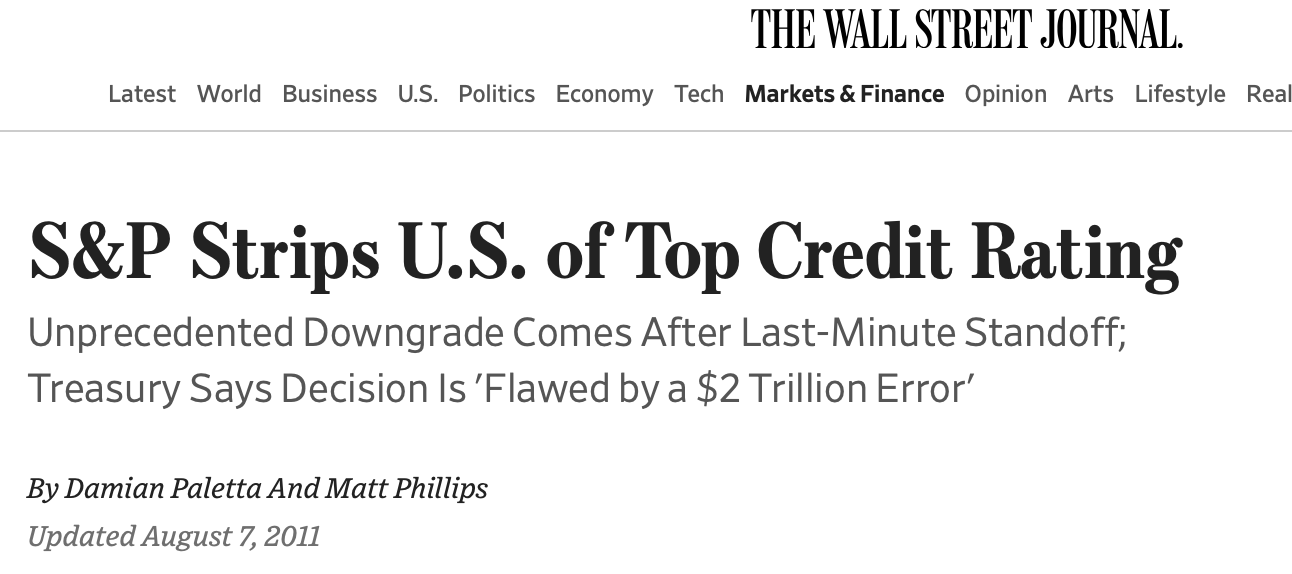
\includegraphics[width=\textwidth]{figures/ch14_2_sp.png}
        \end{column}
        \begin{column}{0.7\textwidth}
            \vspace{1em}
            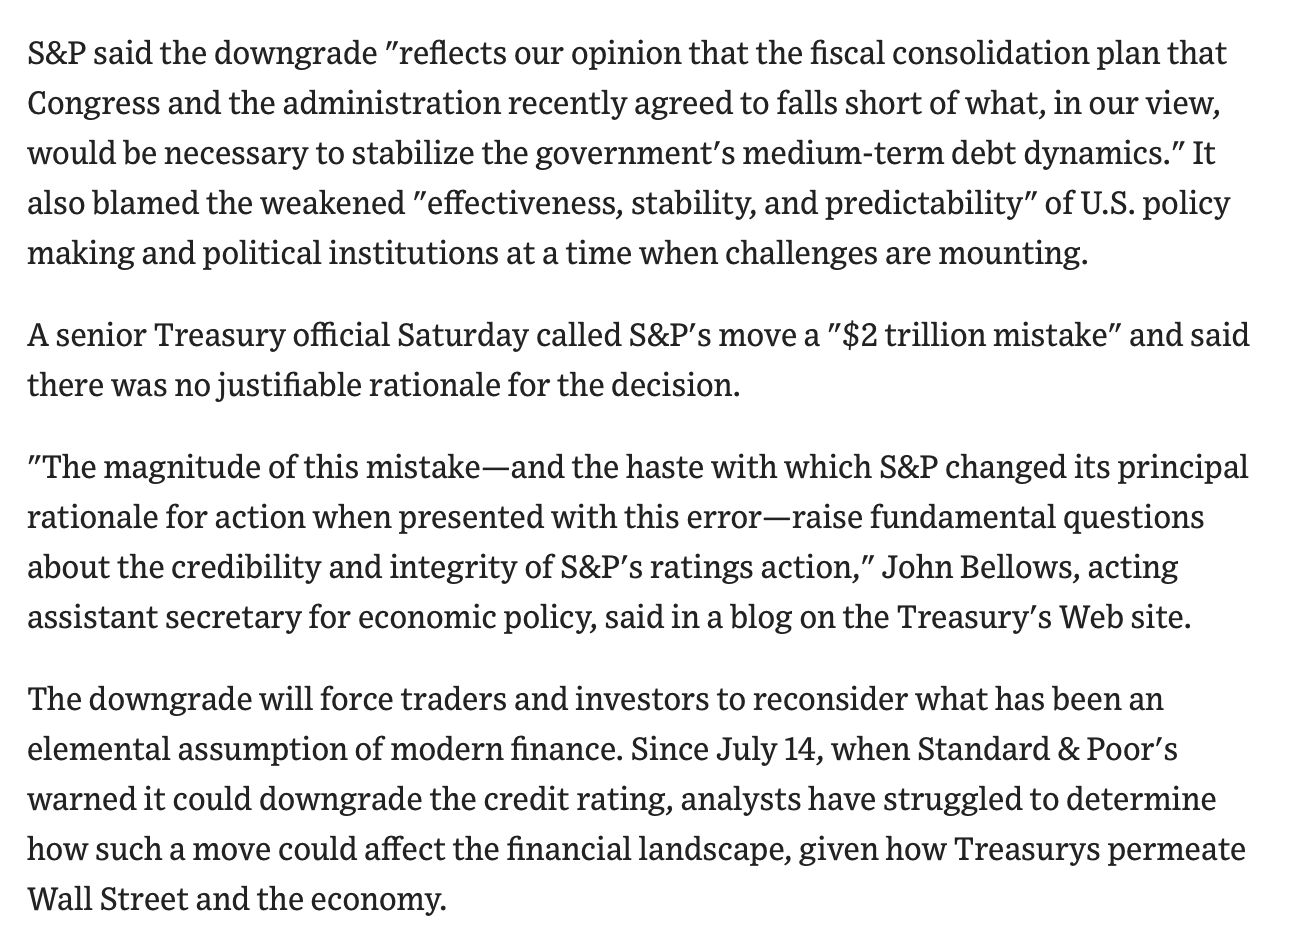
\includegraphics[width=\textwidth]{figures/ch14_2_sp_2.png}
        \end{column}
    \end{columns}

\end{frame}

\begin{frame}[t]
    \frametitle{1. Default Risk }
    \framesubtitle{Credit Ratings}

    \centering
    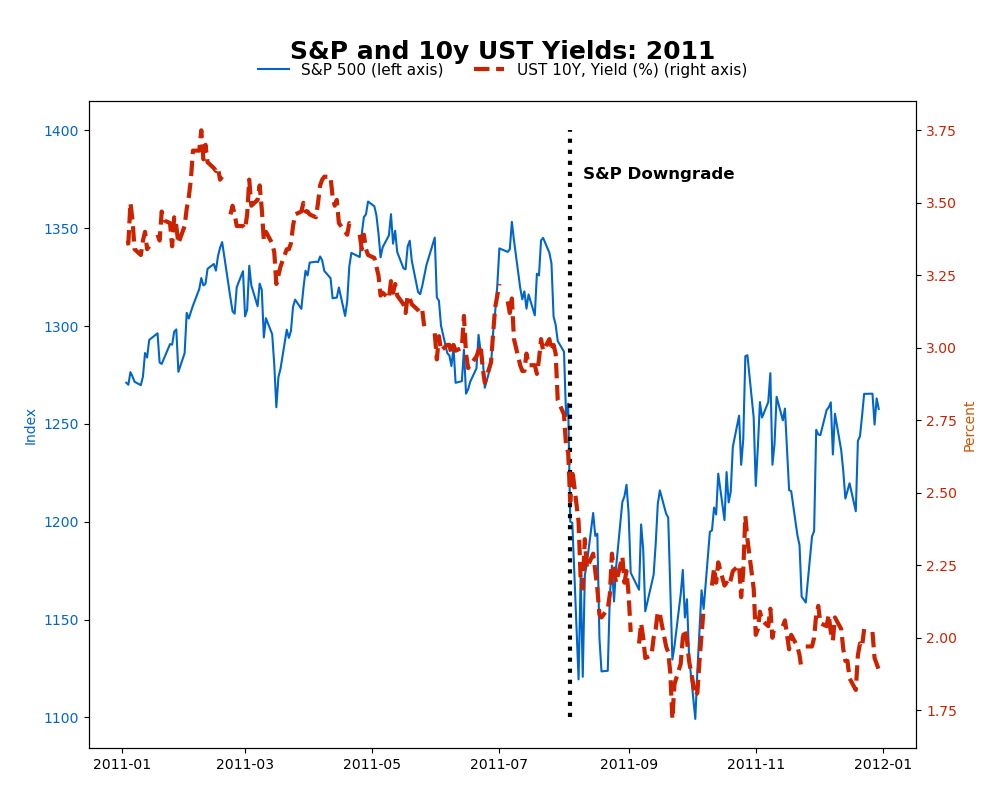
\includegraphics[width=0.8\textwidth]{figures/ch14_sp_downgrade.png}

\end{frame}

\begin{frame}[t]
    \frametitle{2. Tax-exempt Bonds }
    \section{Tax-exempt bonds}

    Interest payments on municipal bonds are exempt from federal income taxes.   These bonds are often referred to as "tax-exempt" or "munis".
    \vspace{1em}
    Considerations:
    \begin{itemize}
        \item The tax exemption makes these bonds more valuable, relative to a similarly-rated taxable bond with the same interest rate.
        \item This shifts the demand curve out, leading to higher prices (lower yields), again relative to a similarly-rated taxable bond with the same interest rate.
        \item What do you think happened to the interest rate on munis when the top tax rate was \textit{lowered} in 2017?   (The top tax rate was lowered from 39.6\% to 37\% that year)
    \end{itemize}
    
\end{frame}

\begin{frame}[t]
    \frametitle{2. Tax-exempt Bonds }

    Yields
    (Indictative, not exact)

    \vspace{-2em}
    \begin{center}
    \end{center}
    \begin{tblr}{
      colspec = { Q[l,wd=2cm] Q[c,wd=2cm] Q[c,wd=5cm, font=\footnotesize] }
    }
    \toprule
    Index & Yields & Comment \\
    \midrule
    UST, 5y & 4.9\% &  na\\
    CA & 4\% & The tax exemption leads to lower yields, relative to USTs \\ 
    NY & 4\% & - \\
    IL & 5.2\% & The default risk outweighs the benefit of the tax exemption \\
    PR & 7\% &  - \\
    \bottomrule
    \end{tblr}
    
\end{frame}  

\begin{frame}[t]
    \frametitle{3. The Treasury Yield Curve}
    \section{Treasury Yield Curve}

    \centering
    
\includegraphics[width=0.8\textwidth]{Econ357/figures/yc_2026-09-11.png}

\end{frame}

\begin{frame}[t]
    \frametitle{3. The Treasury Yield Curve}
    \framesubtitle{Duration}

    The prices of bonds with longer time to maturity are more volatile than the prices of bonds with a shorter time to maturity.  (The bond industry jargon is that longer maturity bonds have more "duration.")\\
    \vspace{1em}

    \textbf{Intuition}
    \begin{itemize}
        \item Look again at the bond price equation.   Note that for the final term, the $(1+y)$ in the denominator is raised to the power $T$, where $T$ is years to maturity.   For the same change in $y$, bonds with a larger $T$ will therefore have a larger change in price.
        \item If yields on alternative bonds increase, then the value of a low coupon bond will decrease.  Intuitively, holders of the low coupon bonds are missing out.  For a shorter maturity bonds, this is not good.   But for a longer maturity bond it is very bad, because the investors will be missing out for potentially 30 years.
    \end{itemize}

\end{frame}

\begin{frame}[t]
    \frametitle{3. The Treasury Yield Curve}
    \section{Treasury Yield Curve}

    \centering
    
\includegraphics[width=0.8\textwidth]{Econ357/figures/yc_2026_ytd.png}

\end{frame}

\begin{frame}[t]
    \frametitle{3. The Treasury Yield Curve}
    \section{Treasury Yield Curve}

    \centering
    
\includegraphics[width=\textwidth]{Econ357/figures/02_mkts_5_2s30s_history.png}

\end{frame}

\begin{frame}[t]
    \frametitle{3. The Treasury Yield Curve}
    \section{Treasury Yield Curve}

    \centering
    
\includegraphics[width=\textwidth]{Econ357/figures/02_mkts_5_tlt.png}

\end{frame}

\begin{frame}[t]
    \frametitle{3. The Treasury Yield Curve}

    Explanations for the slope of the Treasury Yield Curve:
    \begin{itemize}
        \item \textbf{Expectations Hypothesis}
            \begin{itemize}
                \item Yields will reflect the expectations for the future path of short term interest rates.  For example, if short term interest rates are expected to fall over the next year, yields on one year bonds will be lower than yields on 1 month bonds.
            \end{itemize}
        \item \textbf{Market Segmentation}
            \begin{itemize}
                \item Bonds of different maturities are not substitutes.   Differences in demand for certain maturities can raise/lower the yields on those maturities, relative to yields on other maturity bonds.
            \end{itemize}
        \item \textbf{Risk Premium (or Liqudity Premium)}
            \begin{itemize}
                \item Bonds of different maturities have different levels of risk.  Specifically, longer term bonds are more volatile.   Investors may demand a discount to hold more volatile bonds.
            \end{itemize}
    \end{itemize}

\end{frame}

\begin{frame}[t]
    \frametitle{3. The Treasury Yield Curve}

    \centering
    
\includegraphics[width=0.8\textwidth]{Econ357/figures/02_mkts_5_recession3.png}

\end{frame}

\begin{frame}[t]
    \frametitle{3. The Treasury Yield Curve}

    \centering
    
\includegraphics[width=\textwidth]{Econ357/figures/02_mkts_5_recession1.png}

\end{frame}

\begin{frame}[t]
    \frametitle{3. The Treasury Yield Curve}

    \centering
    
\includegraphics[width=\textwidth]{Econ357/figures/02_mkts_5_recession2.png}

\end{frame}

\begin{frame}[t]
    \frametitle{3. The Treasury Yield Curve}

    Discussion
    \begin{itemize}
        \item It turned out that there was no recession in 2025, so in this case, the Treasury curve failed as a predictor of a recession.
        \item More generally, should this work?   If the Treasury curve is downward sloping, does that usually mean a recession is coming?
        \item What, specifically, does a downward sloping Treasury curve signify?
    \end{itemize}

\end{frame}

\end{document}